% !TEX root = ../main.tex
\chapter{Metodología e implementación}
\label{cap:metodologia}

Este capítulo integra la metodología adoptada y la descripción detallada del diseño, implementación y procedimiento experimental de las pruebas de concepto (PoC) desarrolladas para comparar algoritmos cuánticos y clásicos en tres familias de problemas: clasificación supervisada, regresión y optimización combinatoria. Para cada caso de uso se evalúan tres tipos de conjuntos de datos: (i) un dataset diseñado con \textbf{estructura cuántica explícita} (\textit{cuántico-nativo}; sintético, generado de modo que el kernel resulta óptimo por construcción, en la línea de los conjuntos de datos con estructura cuántica de \cite{havlicek2019} y \cite{huang2021} ---en este TFM el mapa empíricamente validado es el \texttt{ZZFeatureMap}; la misma lógica de alineación aplica a otros feature maps), (ii) un dataset real de SKG Tecnología, y (iii) un dataset de referencia de dominio público. Esta triple perspectiva permite distinguir los escenarios donde aparece ventaja por \textbf{alineación dato--feature map} de aquellos donde los algoritmos clásicos siguen siendo superiores en la práctica.

% =====================================================================
\section{Metodología general}
% =====================================================================

La metodología adoptada en este trabajo combina un enfoque experimental cuantitativo con un análisis crítico de los resultados desde la perspectiva de la aplicabilidad empresarial. Se articula en las siguientes fases:

\subsection{Fase 1: Selección y preparación de datos}

Se utilizaron conjuntos de datos reales procedentes de una empresa privada, relacionados con problemas de clasificación de clientes y optimización de asignación de recursos. Los datos fueron anonimizados y tratados conforme a las buenas prácticas de protección de datos. En caso necesario, se complementó el análisis con datos sintéticos generados a partir de distribuciones similares para garantizar la robustez de los resultados y preservar la confidencialidad. Los datasets fueron preprocesados siguiendo técnicas estándar de ciencia de datos: normalización, tratamiento de valores ausentes y reducción de dimensionalidad cuando fue necesario \citep{jordan2015}.

\subsection{Fase 2: Implementación de algoritmos}

Los algoritmos cuánticos se implementaron en simulación clásica mediante el framework \textit{Qiskit} (IBM), que permite simular circuitos cuánticos de hasta decenas de qubits en hardware clásico con ruido controlado. Para los problemas de clasificación se implementaron clasificadores basados en kernels cuánticos \citep{schuld2021} y circuitos variacionales (VQC) \citep{cerezo2021}. Para los problemas de optimización se implementó el QAOA con diferentes valores de profundidad $p$ \citep{farhi2014, zhou2020}. Los algoritmos clásicos de referencia se implementaron mediante las bibliotecas estándar de \textit{scikit-learn} y \textit{scipy}.

\subsection{Fase 3: Diseño experimental y evaluación}

Los experimentos se diseñaron siguiendo un protocolo de validación cruzada estratificada para los problemas de clasificación, y un esquema de múltiples ejecuciones con semillas aleatorias controladas para los problemas de optimización. Las métricas de evaluación principales fueron:

\begin{itemize}
    \item \textbf{Clasificación}: exactitud (\textit{accuracy}), precisión, exhaustividad (\textit{recall}) y puntuación F1, junto con el área bajo la curva ROC (AUC-ROC).
    \item \textbf{Detección de anomalías (one-class)}: ROC-AUC y average precision sobre un test con inliers y outliers; el entrenamiento usa solo inliers.
    \item \textbf{Optimización}: valor de la función objetivo alcanzada, razón de aproximación respecto al óptimo clásico conocido y tiempo de convergencia.
    \item \textbf{Eficiencia computacional}: tiempo de ejecución total, número de qubits requeridos, profundidad del circuito y número de evaluaciones de la función objetivo.
    \item \textbf{Escalabilidad}: evolución del rendimiento en función del tamaño del problema, evaluada mediante experimentos con instancias de tamaño creciente.
\end{itemize}

\subsection{Fase 4: Diseño del prototipo híbrido}

A partir de los resultados obtenidos, se diseñó un flujo de trabajo conceptual que integra el módulo cuántico de mejor rendimiento dentro de una arquitectura de análisis de datos clásica. Este prototipo ilustra los puntos de integración entre componentes cuánticos y clásicos, los requisitos de interfaz y las condiciones de activación del módulo cuántico, proporcionando una visión práctica orientada a la adopción tecnológica futura \citep{cerezo2021}.

Para cada caso de uso se evalúan tres tipos de conjuntos de datos: (i) un dataset diseñado con estructura cuántica explícita (\textit{cuántico-nativo}), (ii) un dataset real de SKG Tecnología, y (iii) un dataset de referencia de dominio público. Esta triple perspectiva permite distinguir los escenarios donde la computación cuántica ofrece ventaja teórica genuina de aquellos donde los algoritmos clásicos siguen siendo superiores en la práctica.

\begin{figure}[ht]
\centering
\begin{tikzpicture}[font=\small,
    fase/.style={rectangle, rounded corners=5pt, very thick,
                 minimum width=9.5cm, minimum height=1.5cm,
                 align=center, inner sep=9pt},
    arr/.style={->, very thick, >=stealth}]
  \node[fase, draw=blue!60!black, fill=blue!9] (f1) {
    \textbf{Fase 1 — Selección y preparación de datos}\\[3pt]
    {\scriptsize Datasets cuántico-nativo, SKG Tecnología y referencia pública
     $\cdot$ Normalización $\cdot$ PCA}
  };
  \node[fase, draw=orange!60!black, fill=orange!9, below=0.6cm of f1] (f2) {
    \textbf{Fase 2 — Implementación de algoritmos}\\[3pt]
    {\scriptsize QSVM $\cdot$ QK-SVR $\cdot$ QAOA $\cdot$ VQE
     $\cdot$ Gradient Boosting $\cdot$ Random Forest}
  };
  \node[fase, draw=teal!60!black, fill=teal!9, below=0.6cm of f2] (f3) {
    \textbf{Fase 3 — Diseño experimental y evaluación}\\[3pt]
    {\scriptsize Validación cruzada $\cdot$ Accuracy $\cdot$ F1-score
     $\cdot$ $R^2$ $\cdot$ AUC-ROC $\cdot$ Escalabilidad}
  };
  \node[fase, draw=violet!60!black, fill=violet!9, below=0.6cm of f3] (f4) {
    \textbf{Fase 4 — Prototipo de arquitectura híbrida}\\[3pt]
    {\scriptsize Integración cuántico-clásica $\cdot$ Criterios de activación
     $\cdot$ Framework QCR}
  };
  \draw[arr] (f1.south) -- (f2.north);
  \draw[arr] (f2.south) -- (f3.north);
  \draw[arr] (f3.south) -- (f4.north);
\end{tikzpicture}
\caption{Flujo metodológico del estudio comparativo en cuatro fases. La Fase~1 establece y pre-procesa los conjuntos de datos; la Fase~2 implementa los algoritmos cuánticos y sus contrapartes clásicas; la Fase~3 evalúa el rendimiento mediante métricas estándar; la Fase~4 sintetiza los resultados en un prototipo de arquitectura híbrida aplicable a SKG Tecnología.}
\label{fig:metodologia_fases}
\end{figure}

% =====================================================================
\section{Entorno tecnológico y arquitectura experimental}
% =====================================================================

Todos los experimentos se ejecutaron en simulación clásica exacta mediante \textit{Qiskit} 2.x \citep{Qiskit} (2.3.0 en el entorno del autor y 2.6.1 en la reejecución; véase la Tabla~\ref{tab:entornos}, Anexo~\ref{anx:entorno}, para todas las versiones), empleando el \texttt{StatevectorSimulator} que evalúa circuitos cuánticos de manera determinista y sin ruido, aislando el efecto del algoritmo cuántico de las imperfecciones del hardware real. Los modelos clásicos se implementaron con \textit{scikit-learn} y \textit{XGBoost}. El entorno del autor fue Python~3.14 sobre una máquina Apple M-series con 16~GB de RAM, y la reejecución se hizo con Python~3.12.3 sobre Linux (Tabla~\ref{tab:entornos}). Todos los experimentos están disponibles en notebooks Jupyter reproducibles.

La elección del simulador de vector de estados garantiza exactitud matemática, pero no captura el ruido cuántico inherente al hardware NISQ real. Esto constituye simultáneamente una fortaleza metodológica ---se evalúa el potencial teórico del algoritmo--- y una limitación práctica: los resultados en hardware real serán necesariamente inferiores debido a la decoherencia y los errores de puerta. Esta distinción se aborda explícitamente en cada caso de uso.

% =====================================================================
\section{Caso de uso 1: Clasificación supervisada con kernel cuántico}
% =====================================================================

\subsection{Descripción del problema}

El primer caso de uso aborda la clasificación binaria supervisada, comparando el QSVM (Quantum Support Vector Machine con kernel cuántico) frente a cuatro clasificadores clásicos de referencia: Gradient Boosting, Random Forest, SVM-RBF y Regresión Logística. La hipótesis central, motivada por \cite{liu2021} y \cite{huang2021}, es que cuando las etiquetas de clase se derivan de una función cuántica alineada con el mapa de características, el kernel cuántico puede aprender el problema con mayor precisión que los clasificadores clásicos. \cite{liu2021} demuestran una separación rigurosa solo para un problema construido sobre el logaritmo discreto, y \cite{huang2021} muestran que la separación exige una diferencia geométrica grande; el dataset de este trabajo es mucho más sencillo (2 qubits, simulable clásicamente) y solo ilustra el mecanismo. Esta asimetría tiene su origen en la diferencia entre el \textbf{espacio de representación} clásico ---el espacio euclídeo $\mathbb{R}^d$ donde operan los clasificadores convencionales--- y el espacio de Hilbert $\mathcal{H}$ al que accede el kernel cuántico a través del mapa de características $\phi\colon \mathbb{R}^d \rightarrow \mathcal{H}$; la similitud en $\mathcal{H}$, medida por el kernel de fidelidad $\kappa(x_i, x_j)=|\langle\phi(x_i)|\phi(x_j)\rangle|^2$, solo puede reproducirse en general mediante una simulación cuyo coste crece exponencialmente con el número de qubits; con los 2 qubits de este trabajo la simulación es trivial. Esta observación motiva la pregunta central del Capítulo~\ref{cap:investigacion_original}: si un dataset real no tiene estructura cuántica nativa, \textquestiondown{}puede transformarse a un espacio de representación $\mathcal{Z}$ adecuado, resolverse con modelos cuánticos en ese espacio, y mapear el resultado de vuelta al espacio original? Esta hipótesis se formaliza como la Conjetura~\ref{conj:qcr} del espacio de representación cuántico-compatible.

% ---
\subsection{Dataset 1: Cuántico-nativo}

Algunas figuras y notebooks conservan la etiqueta histórica «Liu 2021» para este dataset; se refiere a este conjunto sintético y no al problema basado en el logaritmo discreto de \cite{liu2021}.

\paragraph{Descripción y justificación.}
Siguiendo una construcción análoga a la del conjunto de datos de \cite{havlicek2019}, y no el problema basado en el logaritmo discreto de \cite{liu2021}, se generó un dataset sintético donde las etiquetas binarias se definen mediante la expectación de un observable cuántico de Pauli:
\begin{equation}
  y_i = \text{sgn}\!\bigl(\langle\phi(x_i)|\,Z \otimes Z\,|\phi(x_i)\rangle\bigr)
\end{equation}
donde $|\phi(x_i)\rangle$ es el estado cuántico codificado por un \texttt{ZZFeatureMap} de 2 qubits con 2 repeticiones ---el mapa con el que se valida empíricamente el corpus de este TFM, no el único posible---. Por construcción, el kernel de fidelidad $\kappa(x_i, x_j) = |\langle\phi(x_i)|\phi(x_j)\rangle|^2$ es el estimador óptimo del problema. Este dataset no representa un caso práctico real, sino un experimento controlado: la ventaja aparece cuando el feature map está alineado con el generador del dato; ZZ es el mapa que medimos aquí.

\begin{figure}[ht]
\centering
\includegraphics[width=\textwidth]{../POCs/data/output/figures/06_zzfeaturemap_circuit.png}
\caption{Circuito \texttt{ZZFeatureMap} de 2 qubits y 2 repeticiones empleado como mapa de codificación de datos. Las puertas $R_Z(\lambda)$ codifican las features individuales $x_j$; las secuencias $\text{CNOT}$-$R_Z$-$\text{CNOT}$ codifican las interacciones cruzadas $x_j(\pi - x_k)$, que generan la no-linealidad cuántica que define el kernel $\kappa(x_i, x_j)$.}
\label{fig:zzfeaturemap_circuit}
\end{figure}

\paragraph{Procedimiento experimental.}
\begin{enumerate}
  \item \textbf{Generación del dataset}: 200 muestras $(x_i \in [-\pi, \pi]^2, y_i \in \{0, 1\})$ con \texttt{ZZFeatureMap} como función generadora de etiquetas (signo de $\langle ZZ\rangle$); partición estratificada de 140 entrenamiento y 60 test.
  \item \textbf{Preprocesamiento}: Las entradas se generan directamente en $[-\pi, \pi]^2$ para la codificación angular de las puertas de rotación; el análisis de escalabilidad (300 muestras) las reescala además con \texttt{MinMaxScaler} a ese rango.
  \item \textbf{Construcción del kernel}: \texttt{FidelityQuantumKernel} con \texttt{ComputeUncompute} como estimador de fidelidad y \texttt{StatevectorSampler} como backend. La matriz de kernel de entrenamiento ($140 \times 140$) tiene $19{,}600$ entradas, cada una la fidelidad entre dos estados de 2 qubits.
  \item \textbf{Entrenamiento}: \texttt{SVC(kernel=``precomputed'', C=1.0)} con la matriz de kernel cuántico. Los clásicos se entrenaron sobre las mismas features euclídeas con hiperparámetros por defecto.
  \item \textbf{Análisis de escalabilidad}: Experimentos adicionales con $n \in \{30,\allowbreak 50,\allowbreak 80,\allowbreak 100,\allowbreak 140,\allowbreak 180\}$ para comprobar si la ventaja depende del tamaño de entrenamiento: el Notebook~01 usa una partición por tamaño y el módulo \texttt{qml\_v2.scalability} lo repite 10 veces (Capítulo~\ref{cap:evaluacion}).
  \item \textbf{Evaluación}: Accuracy, F1-score y matriz de confusión sobre test ($n=60$).
\end{enumerate}

\paragraph{Resultados preliminares.}
El QSVM alcanzó una exactitud del \textbf{91.7\%}, frente al 53.3\% del mejor clasificador clásico (SVM polinomial de grado 3; SVM-RBF: 46.7\%, Gradient Boosting: 51.7\%, SVM lineal: 45.0\%): \textbf{ventaja de +38.3 pp}. El análisis de escalabilidad del notebook muestra una ventaja positiva en todos los tamaños $n \in [30, 180]$ (una partición por tamaño), con una media de +40.9 pp y un máximo de +48.9 pp para $n=50$.

\paragraph{Ventajas identificadas.}
\begin{itemize}
  \item El kernel cuántico captura exactamente la estructura del espacio de Hilbert que define las etiquetas, produciendo una ventaja amplia que es esperable por construcción, al coincidir mapa y generador de etiquetas.
  \item La ventaja es positiva en todos los tamaños de muestra evaluados; repetida 10 veces por tamaño, es de $+27.1$ a $+37.6$~pp, con intervalos de confianza del 95\% que excluyen el cero y creciente con $n$.
  \item El resultado es coherente con la idea, formalizada por \cite{liu2021} y \cite{huang2021}, de que la ventaja requiere alineación entre kernel y etiquetas; no reproduce la separación rigurosa de \cite{liu2021}, que no es simulable clásicamente.
\end{itemize}

\paragraph{Limitaciones identificadas.}
\begin{itemize}
  \item El dataset es artificial y diseñado a medida para el kernel cuántico; no existe evidencia de que los datos del mundo real presenten esta estructura.
  \item El coste computacional de construir la matriz de kernel escala como $O(n^2)$ en evaluaciones de circuito, haciendo prohibitivo el entrenamiento con $n > 1{,}000$ en simulación.
  \item La simulación exacta no captura ruido cuántico; en hardware NISQ real, la fidelidad disminuiría y la ventaja podría reducirse o desaparecer con la profundidad de circuito actual.
\end{itemize}

% ---
\subsection{Dataset 2: SKG Tecnología (incidentes de movilidad urbana, NUSE Bogotá)}

\paragraph{Descripción y justificación.}
Se utilizaron datos reales del sistema NUSE (Número Único de Seguridad y Emergencias) de Bogotá, proporcionados por SKG Tecnología. El dataset contiene 27.326 registros de incidentes de movilidad con dos clases: incidente \textit{simple} (sin lesionados, $n=12{,}035$, 44\%) e incidente \textit{con lesionado} ($n=15{,}291$, 56\%). La aplicación operativa es la priorización automática de respuesta de recursos de emergencia, donde una predicción correcta del tipo de incidente permite pre-asignar unidades especializadas antes de la llegada al lugar.

\paragraph{Procedimiento experimental.}
\begin{enumerate}
  \item \textbf{Carga y limpieza}: 27.326 registros con gravedad simple o con lesionado; imputación de los valores ausentes del número de implicados con la mediana. Variables seleccionadas, todas numéricas: prioridad, tipo de incidente, zona, orientación, número de implicados, latitud y longitud (7 variables).
  \item \textbf{Estandarización}: \texttt{StandardScaler} sobre la submuestra (el escalado y la PCA se ajustan con las 360 instancias antes de dividir en entrenamiento y test, de modo que el test participa en esa transformación no supervisada).
  \item \textbf{Reducción dimensional (PCA)}: El kernel cuántico opera sobre 2 qubits, por lo que se redujo a 2 dimensiones. Varianza explicada por los dos primeros componentes: \textbf{84.6\%} (pérdida: 15.4\%).
  \item \textbf{Submuestreo balanceado}: Submuestra de $n_{\text{train}} = 240$ y $n_{\text{test}} = 120$ instancias balanceadas, impuesta por el coste cuadrático del kernel.
  \item \textbf{Escalado al rango cuántico}: Componentes PCA escaladas a $[-\pi, \pi]$.
  \item \textbf{Evaluación}: exactitud sobre el test de 120 instancias para el QSVM y sobre el 20\% de reserva (5\,466 registros) para los clásicos, que se entrenan con el 80\% restante (21\,860).
\end{enumerate}

\paragraph{Resultados preliminares.}
El QSVM obtuvo exactitud del \textbf{55.0\%}, frente al \textbf{59.5\%} de SVM-RBF: \textbf{desventaja de $-$4.5 pp}. Gradient Boosting y Random Forest (58.8\%) y la regresión logística (57.0\%) quedaron entre ambos. Ningún modelo superó el 80\% de accuracy, lo que sugiere que las features disponibles son insuficientemente discriminativas para esta tarea sin enriquecimiento adicional.

\paragraph{Ventajas identificadas.}
\begin{itemize}
  \item Demuestra que el QSVM es directamente aplicable a datos reales del sector de movilidad urbana sin modificaciones de implementación, validando la viabilidad técnica del enfoque.
  \item La diferencia de rendimiento es pequeña ($-$4.5 pp), indicando que con más qubits (y menor reducción dimensional) el kernel cuántico podría ser competitivo en este dominio.
  \item Establece una línea base cuantitativa para comparaciones futuras cuando hardware cuántico real de mayor capacidad esté disponible.
\end{itemize}

\paragraph{Limitaciones identificadas.}
\begin{itemize}
  \item La reducción a 2 dimensiones implica una pérdida del 15.4\% de varianza. Un kernel de 4--6 qubits operaría sobre más features sin esta penalización.
  \item El submuestreo a 240 instancias (frente a las 21.860 de entrenamiento de los clásicos) impide que el QSVM aproveche la capacidad estadística del dataset.
  \item Los datos presentan correlaciones temporales y espaciales que el kernel cuántico estacionario no modela explícitamente.
  \item La simulación sin ruido sobreestima el rendimiento cuántico que se obtendría en hardware NISQ real.
\end{itemize}

% ---
\subsection{Dataset 3: Telco Customer Churn (referencia)}

\paragraph{Descripción y justificación.}
Como benchmark de dominio público se empleó el dataset \textit{Telco Customer Churn} (IBM, 7.043 registros, 20 variables predictoras), problema estándar de predicción de abandono de clientes con clase positiva desbalanceada (26.5\% churn). Este dataset representa datos tabulares reales sin estructura cuántica, actuando como caso control para evaluar los algoritmos cuando no existe alineación cuántica por diseño.

\paragraph{Procedimiento experimental.}
\begin{enumerate}
  \item \textbf{Preprocesamiento}: Eliminación de columnas de identificador; imputación de \texttt{TotalCharges} (11 nulos); codificación de categóricas (LabelEncoder y OrdinalEncoder).
  \item \textbf{Reducción dimensional}: PCA a 4 componentes (varianza explicada: 48.5\%) para el QSVM; clásicos sobre las 21 variables (20 originales más dos derivadas, \texttt{charge\_ratio} y \texttt{num\_services}).
  \item \textbf{Submuestreo}: 100 ejemplos de entrenamiento y 50 de test para el QSVM; los clásicos usan la partición completa (5\,634 de entrenamiento, 1\,409 de test). La comparación es por tanto asimétrica (véase la Tabla~\ref{tab:clasif_justa} para el protocolo justo).
  \item \textbf{Gestión del desbalanceo}: \texttt{class\_weight=``balanced''} en SVM-RBF y Random Forest, y \texttt{scale\_pos\_weight} en XGBoost.
  \item \textbf{Evaluación}: Accuracy, precisión, recall y F1 ponderados.
\end{enumerate}

\paragraph{Resultados preliminares.}
El QSVM obtuvo exactitud del \textbf{76.0\%} (F1 ponderado: 0.656), frente al \textbf{79.8\%} del Gradient Boosting (F1 ponderado: 0.789): \textbf{desventaja de $-$3.8 pp}, sobre un test de solo 50 ejemplos para el QSVM. Bajo el protocolo justo del Capítulo~\ref{cap:evaluacion}, la desventaja en Telco es de $-23.8$~pp.

\paragraph{Ventajas identificadas.}
\begin{itemize}
  \item El QSVM alcanza una exactitud del 76.0\% con solo 4 componentes PCA, pero sobre un test de 50 ejemplos (una desviación de un solo ejemplo equivale a 2~pp), por lo que esta cifra no permite concluir que el kernel cuántico actúe como regularizador.
  \item El resultado confirma la validez del diseño experimental: la ausencia de estructura cuántica produce la victoria clásica esperada, lo que valida la metodología comparativa.
\end{itemize}

\paragraph{Limitaciones identificadas.}
\begin{itemize}
  \item La reducción de 21 variables a 4 componentes PCA (48.5\% de varianza explicada) penaliza al QSVM; los clásicos usan toda la información disponible, lo que hace la comparación asimétrica en dimensionalidad de entrada.
  \item El dataset presenta desbalanceo de clase que el QSVM gestiona con menos flexibilidad que los métodos basados en árboles de decisión.
  \item La submuestra cuántica (100 ejemplos de entrenamiento y 50 de test) es insuficiente para estimar con robustez estadística la distribución del churn.
\end{itemize}

% ---
\subsection{Análisis comparativo directo: QSVM (kernel cuántico) vs.\ SVM-RBF (kernel clásico)}
\label{sec:qsvm_vs_svm_directo}

Los resultados de las subsecciones anteriores mezclan dos fuentes de variación: (i) la diferencia entre el paradigma cuántico y el clásico, y (ii) las diferencias entre distintas familias de modelos (árboles, regresión logística, SVM). Para aislar específicamente la contribución del \emph{kernel cuántico} frente al \emph{kernel clásico}, se realiza aquí un contraste directo entre \textbf{QSVM con ZZFeatureMap} y \textbf{SVM-RBF} bajo condiciones estrictamente controladas: mismo clasificador base (\texttt{SVC}), mismo conjunto de entrenamiento/test, mismos hiperparámetros ($C = 1.0$) y misma reducción dimensional (PCA a 2 componentes en todos los datasets). La única variable modificada es el tipo de kernel.

\begin{table}[ht]
\centering
\caption{Comparativa directa QSVM (kernel cuántico ZZFeatureMap) vs.\ SVM-RBF (kernel clásico). Condiciones controladas: mismo \texttt{SVC} base, $C=1.0$, PCA a 2 componentes, mismas particiones train/test.}
\label{tab:qsvm_vs_svm_directo}
\begin{tabularx}{\linewidth}{>{\raggedright\arraybackslash}Xcccc}
\toprule
\textbf{Dataset} & \textbf{QSVM (Acc)} & \textbf{SVM-RBF (Acc)} & \textbf{$\Delta$ Acc} & \textbf{Ventaja} \\
\midrule
Cuántico-nativo & 0.533 & 0.467 & $+0.067$ & \textbf{QSVM} \\
SKG Incidentes movilidad   & 0.467 & 0.525 & $-0.058$ & SVM-RBF \\
Telco Customer Churn       & 0.735 & 0.747 & $-0.013$ & SVM-RBF (marginal) \\
\bottomrule
\end{tabularx}
\end{table}

\begin{figure}[ht]
\centering
\includegraphics[width=0.95\textwidth]{../POCs/data/output/figures/01_qsvm_vs_svm_directo.png}
\caption{Comparativa directa QSVM (kernel cuántico ZZFeatureMap) vs.\ SVM-RBF (kernel clásico) bajo condiciones controladas idénticas (mismo \texttt{SVC} base, $C=1.0$, PCA a 2 componentes). El eje vertical muestra la exactitud; el signo del $\Delta$ indica ventaja cuántica (positivo) o ventaja clásica (negativo). La ventaja cuántica solo emerge en el dataset con estructura cuántica nativa, confirmando la hipótesis de alineación estructural.}
\label{fig:qsvm_vs_svm_directo}
\end{figure}


\paragraph{Interpretación.}
El contraste directo revela un patrón coherente con la expectativa de \cite{liu2021} y \cite{huang2021} de que la ventaja depende de la alineación entre kernel y datos:

\begin{itemize}
  \item \textbf{Dataset cuántico-nativo:} el kernel cuántico ZZFeatureMap supera al RBF en $+6.7$ pp. Ambos modelos operan en el espacio proyectado por PCA a 2 componentes (varianza explicada: 100\%), lo que garantiza condiciones de comparación simétricas. La diferencia equivale a 4 aciertos sobre 60 puntos de test, con ambos modelos cerca del azar tras la proyección a 2 componentes, por lo que no es estadísticamente concluyente; la evidencia robusta de este régimen es la del Caso~1 (10 repeticiones).

  \item \textbf{Dataset SKG (incidentes de movilidad):} el SVM-RBF supera al QSVM en $5.8$ pp (y GB/RF mantienen la superioridad operativa). Con PCA a 2 componentes y varianza explicada del 63.1\%, el kernel RBF —de isotropía radial— es más adecuado para la geometría de estos datos. Un $\mathcal{Q}(\text{SKG}) = +0.163$ puntual frente a RBF (definición del Notebook~09, Capítulo~\ref{cap:investigacion_original}) \textbf{no} implica que SKG sea cuántico-nativo: bajo $\mathcal{Q}_{\mathrm{rob}}$ el veredicto es clásico, y el bajo rendimiento absoluto ($< 55\%$) sugiere además pérdida discriminativa por la proyección a 2D.

  \item \textbf{Telco Churn:} la diferencia es mínima ($-1.3$ pp) y dentro del margen de variabilidad estadística con el tamaño de muestra utilizado ($n_{\text{train}} = 120$). El score $\mathcal{Q}(\text{Telco}) = -0.228$ predice correctamente la ausencia de ventaja cuántica en este dataset.
\end{itemize}

\paragraph{Conclusión del contraste.}
El diferencial de rendimiento entre el kernel cuántico y el RBF es una función directa de la adecuación estructural del dataset al espacio de Hilbert del circuito, cuantificable mediante el score $\mathcal{Q}(\mathcal{D})$ del Capítulo~\ref{cap:investigacion_original}. Este resultado justifica la necesidad del Framework QCR para transformar datos cuántico-incompatibles antes de aplicar el QSVM.

% =====================================================================
\section{Caso de uso 2: Regresión con kernel cuántico (QK-SVR)}
% =====================================================================

\subsection{Descripción del problema}

El segundo caso de uso evalúa la regresión cuántica mediante QK-SVR (Quantum Kernel Support Vector Regressor) frente a cuatro regressores clásicos: XGBoost, Random Forest, SVR-RBF y Ridge. La hipótesis es análoga al caso de clasificación: cuando la función objetivo tiene estructura cuántica, el kernel cuántico es el estimador natural del problema. Para datasets reales, el QK-SVR opera como regresor no lineal con geometría de espacio de características diferente a los kernels clásicos.

% ---
\subsection{Dataset 1: Cuántico-nativo}

\paragraph{Descripción y justificación.}
Se generó un dataset de regresión donde los valores objetivo son la expectación continua del observable cuántico:
\begin{equation}
  y_i = \langle\phi(x_i)|\,Z \otimes Z\,|\phi(x_i)\rangle \in [-1, 1]
\end{equation}
El kernel cuántico de fidelidad es, por construcción, el estimador natural de esta función: el dato está generado por el mismo mapa que define el kernel.

\paragraph{Procedimiento experimental.}
\begin{enumerate}
  \item \textbf{Generación}: 200 muestras $x_i \in [-\pi,\pi]^2$ con $y_i=\langle ZZ\rangle$ calculado con \texttt{Statevector}; las entradas que recibe el kernel son exactamente aquellas con las que se calculó la etiqueta, y se divide 140/60 (entrenamiento/test, semilla 42).
  \item \textbf{Construcción del kernel}: \texttt{ZZFeatureMap} (2 qubits, \texttt{reps=2}, entrelazamiento completo) y \texttt{FidelityQuantumKernel}.
  \item \textbf{Entrenamiento}: \texttt{SVR(kernel=``precomputed'', C=10.0, epsilon=0.1)} con el kernel cuántico; los clásicos (Ridge, Random Forest, SVR-RBF y SVR-Poly) se entrenan sobre las mismas entradas.
  \item \textbf{Evaluación}: $R^2$ y RMSE sobre el conjunto de test.
\end{enumerate}

\paragraph{Resultados.}
El QK-SVR obtuvo $R^2 = 0.985$ frente a $R^2 = 0.020$ del mejor clásico (SVR-Poly): $\Delta R^2 = +0.965$. Los clásicos no superan el nivel de una predicción constante, mientras que el kernel cuántico reproduce la función porque esta es, por construcción, lineal en su espacio de características.

\paragraph{Ventajas identificadas.}
\begin{itemize}
  \item Es el único dataset de regresión en el que el kernel cuántico supera al mejor clásico, y es precisamente aquel cuyo generador coincide con el mapa de características.
  \item La implementación de regresión cuántica es directamente reutilizable sin modificar la arquitectura del modelo.
\end{itemize}

\paragraph{Limitaciones identificadas.}
\begin{itemize}
  \item No se exploraron otros hiperparámetros; los clásicos podrían mejorar con una búsqueda sobre $C$ y $\varepsilon$.
  \item Una sola partición de 60 puntos de test no permite estimar la incertidumbre de la diferencia; el protocolo justo (10 repeticiones) la acota: $\Delta R^2=+1.002$ con desviación $0.002$ del QK-SVR.
\end{itemize}

% ---
\subsection{Dataset 2: SKG Tecnología (tiempos de viaje en corredores viales, Bogotá)}

\paragraph{Descripción y justificación.}
Se utilizaron los datos históricos de tiempos de viaje en corredores viales de Bogotá (\texttt{bctraveltimes\_history.csv}), con 81.121 registros. La variable objetivo es la velocidad media del vehículo en km/h (media: 26.0, $\sigma = 12.5$ km/h). La aplicación operativa es la predicción de niveles de servicio para la gestión proactiva del tráfico urbano y la asignación dinámica de recursos de respuesta.

\paragraph{Procedimiento experimental.}
\begin{enumerate}
  \item \textbf{Carga y limpieza}: 81.121 registros; eliminación de filas con nulos en \texttt{speed}. Extracción de features temporales de \texttt{read\_time}: hora del día, día de la semana.
  \item \textbf{Feature engineering}: Features finales: \texttt{elapsed\_time}, \texttt{readings}, hora del día, nivel de servicio codificado (\textit{green}=0, \textit{yellow}=1, \textit{red}=2). Total: 4 features.
  \item \textbf{Reducción dimensional}: PCA a 2 componentes (varianza explicada: \textbf{68.6\%}; pérdida: 31.4\%).
  \item \textbf{Submuestreo}: $n_{\text{train}} = 150$, $n_{\text{test}} = 80$ para QK-SVR; entrenamiento completo (64\,896 registros) para clásicos.
  \item \textbf{Escalado}: \texttt{MinMaxScaler} sobre componentes PCA a $[-\pi, \pi]$; target normalizado a $[0,1]$.
  \item \textbf{Evaluación}: $R^2$, RMSE (km/h), MAE (km/h).
\end{enumerate}

\paragraph{Resultados preliminares.}
El QK-SVR obtuvo $R^2 = 0.098$ (RMSE = 11.04 km/h), frente al $R^2 = 0.660$ del Gradient Boosting (RMSE = 7.25 km/h): \textbf{desventaja de $\Delta R^2 = -0.562$}. Un error de 11 km/h no es operativamente útil para la gestión de tráfico.

\paragraph{Ventajas identificadas.}
\begin{itemize}
  \item El QK-SVR puede aportar diversidad en un ensemble heterogéneo de modelos, dado que captura patrones geométricos distintos a los que explotan los árboles de decisión.
  \item El experimento confirma la aplicabilidad técnica directa del método a series de movilidad urbana sin adaptaciones de arquitectura.
\end{itemize}

\paragraph{Limitaciones identificadas.}
\begin{itemize}
  \item La varianza explicada por PCA a 2 componentes es del 68.6\%, con pérdida significativa de patrones temporales y de servicio. Un kernel de 4 qubits retendría más información.
  \item Con 81.121 registros disponibles, el submuestreo a 150 instancias de entrenamiento supone usar el 0.23\% de las 64\,896 observaciones de entrenamiento de los clásicos, lo que impide una comparación equitativa con los clásicos.
  \item Los datos presentan autocorrelación temporal fuerte que el kernel cuántico estacionario no modela, a diferencia de modelos con features de rezago o arquitecturas secuenciales.
  \item La correlación entre \texttt{levelofservice} y \texttt{speed} es casi determinista (rojo $\approx$ lento, verde $\approx$ rápido), una relación que los árboles capturan perfectamente sin necesidad de un kernel cuántico.
\end{itemize}

% ---
\subsection{Dataset 3: Friedman \#1 (referencia)}
\label{sec:friedman}

\paragraph{Descripción y justificación.}
Como benchmark estándar en regresión no lineal se utilizó el dataset sintético Friedman \#1 \citep{friedman1991}:
\begin{equation}
  y = 10\sin(\pi x_1 x_2) + 20(x_3 - 0.5)^2 + 10x_4 + 5x_5 + \varepsilon, \quad \varepsilon \sim \mathcal{N}(0, 1)
\end{equation}
La componente $\sin(\pi x_1 x_2)$ es una interacción multiplicativa oscilatoria; el término $\phi(x_i,x_j)=(\pi-x_i)(\pi-x_j)$ del \texttt{ZZFeatureMap} motivó probar si el kernel cuántico la captura, pero el dataset no está generado por ese mapa.

\paragraph{Procedimiento experimental.}
\begin{enumerate}
  \item \textbf{Generación}: \texttt{make\_friedman1(n\_samples=300, noise=1.0)}, 5 características y partición 70/30 (210/90, semilla 42).
  \item \textbf{Escalado}: estandarización y reescalado a $[0,\pi]$; sin reducción de dimensión (5 qubits, \texttt{ZZFeatureMap} con \texttt{reps=2}).
  \item \textbf{QK-SVR}: por coste del simulador se usan los primeros 150 puntos de entrenamiento y 60 de test; $(C,\varepsilon)$ se elige por rejilla maximizando $R^2$ sobre esos 60 puntos de test, lo que favorece al QK-SVR frente a los clásicos (sin ajuste) y no cambia el signo del resultado.
  \item \textbf{Clásicos}: regresión lineal, Random Forest y XGBoost entrenados con las 210 muestras y evaluados sobre los mismos 60 puntos.
\end{enumerate}

\paragraph{Resultados preliminares.}
El QK-SVR obtuvo $R^2 = -0.151$ (RMSE = 4.83) frente a $R^2 = 0.777$ de XGBoost (RMSE = 2.13): $\Delta R^2 = -0.928$.

\paragraph{Lectura.}
El kernel cuántico no es competitivo en este benchmark clásico: queda por debajo incluso de la regresión lineal ($R^2=0.641$) y de Random Forest ($R^2=0.704$). El resultado es coherente con el criterio de alineación entre mapa y generador: Friedman~\#1 no está generado por el \texttt{ZZFeatureMap}.

\paragraph{Limitaciones identificadas.}
\begin{itemize}
  \item El QK-SVR se entrena con 150 puntos y se evalúa con 60, y sus hiperparámetros se eligen sobre ese mismo test; los clásicos no tuvieron ajuste equivalente. Ambas decisiones favorecen al kernel cuántico, de modo que el signo del resultado no se explica por ellas.
  \item Una única partición no proporciona intervalo de confianza.
\end{itemize}

% =====================================================================
\section{Caso de uso 3: Optimización de asignación de recursos (QAOA)}
% =====================================================================

\subsection{Descripción del problema y formulación QUBO}

El QAOA \citep{farhi2014} se aplicó al problema de asignación de agentes a tareas, núcleo de la gestión de flotas de SKG Tecnología. Dada una matriz de costes $C\in\mathbb{R}^{n\times n}$, se busca una permutación que minimice
\begin{equation}
  \min_{x\in\{0,1\}^{n\times n}} \sum_{i,j} C_{ij}\,x_{ij}
  \quad\text{s.a.}\quad \sum_j x_{ij}=1\;\forall i,\qquad \sum_i x_{ij}=1\;\forall j,
\end{equation}
donde $x_{ij}=1$ indica que el agente $j$ atiende la tarea $i$. Las restricciones se incorporan al Hamiltoniano mediante \texttt{QuadraticProgramToQubo} de Qiskit Optimization; para $n=3$ el problema usa nueve qubits.

\subsection{Procedimiento experimental}

El módulo \texttt{POCs/qml\_v2/optimization.py} aplica el mismo modelo a todos los métodos:
\begin{enumerate}
  \item \textbf{Instancias}: cinco matrices $3\times3$ con costes uniformes en $[1,10]$ y semillas 42--46.
  \item \textbf{Referencia exacta}: algoritmo húngaro y PuLP/CBC; deben coincidir.
  \item \textbf{Greedy}: cada tarea toma el agente libre de menor coste.
  \item \textbf{QAOA}: \texttt{QAOA} de Qiskit con $p=1$, \texttt{StatevectorSampler} y COBYLA (80 iteraciones máximas, 3 reinicios); la solución se decodifica de las variables binarias y se evalúa con el coste original, no con la energía del QUBO.
  \item \textbf{Métricas}: coste, brecha frente al óptimo exacto, factibilidad y tiempo.
\end{enumerate}

\paragraph{Resultados.}
QAOA alcanza el óptimo exacto en las cinco instancias; Greedy lo falla en una ($+35.2\%$) y queda en media un $7.0\%$ por encima. Los métodos exactos tardan menos de $0.02$~s frente a cientos de segundos de la simulación de QAOA. El análisis se presenta en el Capítulo~\ref{cap:evaluacion}.

\paragraph{Limitaciones identificadas.}
\begin{itemize}
  \item Con $n=3$ hay solo seis soluciones factibles; el resultado valida el \emph{pipeline} pero no discrimina entre métodos potentes.
  \item La formulación usa $n^2$ variables binarias; $n=6$ ya requiere 36 qubits, fuera del alcance de la simulación de vector de estados.
  \item El problema de asignación es polinómico, por lo que no es un candidato natural a ventaja cuántica; sirve como banco de pruebas del flujo QUBO--QAOA.
\end{itemize}

% =====================================================================
\section{Caso de uso 4: Optimización de portafolio (VQE/QAOA)}
% =====================================================================

Se aplicó VQE (\textit{Variational Quantum Eigensolver}) y QAOA a la selección de tres activos entre seis, formulada como el problema cuadrático binario $\min_x\, q\,x^\top\Sigma x-\mu^\top x$ sujeto a $\sum_i x_i=3$, con $q=0.5$ y $\mu,\Sigma$ estimados con retornos logarítmicos diarios anualizados (252 sesiones) de EC, CIB, AAPL, MSFT, GOOGL y AMZN (cierres ajustados descargados de Yahoo Finance, 2022--2023; los log-retornos no dependen del factor constante con que Yahoo reajusta los cierres tras un dividendo). La restricción de presupuesto se incorpora al Hamiltoniano de Ising con un término de penalización (\texttt{QuadraticProgramToQubo}). El óptimo exacto se obtiene por fuerza bruta sobre las $\binom{6}{3}=20$ carteras factibles y se contrasta con una selección voraz (Greedy).

El protocolo \texttt{qml\_v2.portfolio} usa para ambos métodos 10 semillas independientes, \texttt{TwoLocal} ($R_Y$+CZ, 3 capas) para VQE y \texttt{QAOAAnsatz} con $p=3$ para QAOA, COBYLA como optimizador y la cadena más probable de 4\,096 disparos como solución. Se evaluaron dos configuraciones: penalización 10 con 5 reinicios y 300 evaluaciones por reinicio, y penalización 0.01 (la del notebook original) con un solo inicio y 200 evaluaciones. Una ejecución solo cuenta si es factible y se evalúa en el problema original, no en la energía penalizada. Los resultados se discuten en el Capítulo~\ref{cap:evaluacion}.

\paragraph{Limitaciones identificadas.}
\begin{itemize}
  \item Para $n > 6$ activos, el número de qubits necesarios crece rápidamente y la simulación exacta se vuelve costosa.
  \item La formulación cuadrática no captura restricciones de mercado como liquidez mínima, lotes enteros o costes de transacción variables.
\end{itemize}

% =====================================================================
\section{Caso de uso 5: Problema del viajante cerrado (TSP justo)}
\label{sec:caso5_tsp}
% =====================================================================

La versión original del Notebook~05 comparaba instancias de distinto tamaño y puntuaba QAOA con energía Ising y bitstrings a menudo infactibles; además, su codificación de 16 qubits (sin fijar el depósito) no puede reejecutarse con el simulador de vector de estados (la evolución densa exige 64~GiB). El Notebook~05 actual usa el protocolo QML~v2 (\texttt{POCs/qml\_v2/tsp\_optimization.py}), que corrige esos problemas: \textbf{TSP cerrado de un vehículo} (no VRP), misma matriz de distancias $D$ y misma longitud de tour $L(\pi)$ para todos los solvers.

\subsection{Protocolo experimental justo}

\begin{itemize}
  \item \textbf{Referencia exacta:} fuerza bruta $(n-1)!$ con depot fijo.
  \item \textbf{Clásicos:} Nearest Neighbor, NN multi-start, \textbf{NN+2-opt} (búsqueda local fuerte), Random-tour.
  \item \textbf{SA-QUBO:} Simulated Annealing sobre el QUBO de Lucas con $(n-1)^2$ variables (depot fijo), coste reportado en km (o Euclidean), nunca energía Ising.
  \item \textbf{QAOA:} mismas igualdades QP + decodificación por variables nombradas; coste = $L(\pi)$ del tour factible.
\end{itemize}

Configuración reportada: $n=4$ ciudades, depot fijo $\Rightarrow$ 9 qubits, $p=1$, familia Colombia (distancias reales entre capitales) y réplicas Euclidean.

\subsection{Resultados (Colombia \texorpdfstring{$n=4$}{n=4})}

\begin{table}[ht]
\centering
\small
\begin{tabular}{lcc}
\hline
\textbf{Solver} & \textbf{Coste (km)} & \textbf{Gap vs exacto} \\
\hline
BruteForce-opt & \textbf{1867.6} & 0 \\
\textbf{NN+2-opt} & \textbf{1867.6} & 0 \\
\textbf{QAOA-$p$1} & \textbf{1867.6} & 0 (factible) \\
SA-QUBO & 1867.6 & 0 \\
NearestNeighbor & 2124.6 & $+13.8\%$ \\
\hline
\end{tabular}
\caption{Caso~5, Colombia $n=4$. 2-opt recupera el óptimo que el NN plano pierde; QAOA iguala al exacto bajo protocolo justo.}
\label{tab:tsp_colombia}
\end{table}

Sobre las 12 capitales del Notebook~05, donde el óptimo exacto ($11!=39\,916\,800$ tours) queda fuera del cuaderno, NN+2-opt reduce el tour del NN de 2564.1 a 2230.6~km. En réplicas Euclidean ($n=4$, 3 instancias), QAOA y NN+2-opt alcanzan gap~$0$ frente al exacto; SA-QUBO es más débil en media (gap~$\approx 0.12$).

\paragraph{Lectura.}
El valor del Caso~5 es de \textbf{protocolo y modelado QUBO/QAOA}, no de speedup: a $n=4$ el clásico fuerte (NN+2-opt) ya es óptimo y milisegundos. QAOA demuestra que, con decodificación correcta, recupera $L(\pi)$ óptimo; no sustituye a 2-opt en esta escala. VRP con ventanas temporales queda fuera de alcance (Capítulo~\ref{cap:futuro}).

\paragraph{Limitaciones.}
\begin{itemize}
  \item Codificación Lucas: $(n-1)^2$ qubits con depot fijo; $n=15$ ya exige cientos de qubits solo de variables.
  \item Para $n \gtrsim 20$, heurísticas clásicas (LKH, SA clásico) dominan calidad y tiempo en simulación NISQ.
\end{itemize}

% =====================================================================
\section{Caso de uso 6: Análisis de umbral de ventaja del kernel cuántico}
% =====================================================================

Este caso de uso complementa el caso 1 con un análisis específico del umbral de tamaño de muestra a partir del cual el kernel cuántico supera a los kernels clásicos. Con la motivación teórica de \cite{liu2021} y \cite{huang2021}, se evaluó el régimen de ventaja en el dataset cuántico-nativo ($n\in\{50,80,100,120,150\}$ muestras, partición 70/30 única por tamaño) y se contrastó con controles reales (SKG, Telco) donde \textbf{no} hay alineación mapa--generador.

\paragraph{Resultados.}
En el dataset cuántico-nativo ($n=150$, 45 puntos de test), el QSVC obtuvo 68.9\% frente al 60.0\% del mejor clásico (SVM polinomial): \textbf{+8.9 pp}, es decir, cuatro aciertos más sobre una única partición, por lo que la diferencia no es estadísticamente concluyente por sí sola; la evidencia robusta de este régimen es la del Caso~1 (protocolo con 10 repeticiones). SKG (Incidentes Bogotá) \textbf{no} es cuántico-nativo: QSVC 56.7\% frente a 60.7\% del mejor clásico ($-4.0$~pp). Telco tampoco: QSVM 76.0\% frente a 79.8\% de Gradient Boosting (\textbf{$-3.8$~pp}); el baseline operativo es GB/RF, no un RBF aislado en un subconjunto pequeño. Una versión previa del Notebook~06 estimaba el kernel con un muestreador de 1024 \emph{shots} sin semilla, de modo que el mismo experimento no era reproducible entre ejecuciones; se sustituyó por el cálculo exacto de la fidelidad, que es determinista y coincide con el resto de cuadernos.

\paragraph{Limitaciones identificadas.}
\begin{itemize}
  \item El umbral de ventaja depende fuertemente de la estructura del dataset; no es posible determinar a priori si un dataset real exhibirá ventaja cuántica sin experimentación específica.
  \item El coste cuadrático de la matriz de Gram limita el análisis: con $n\le150$ muestras el QSVC tarda entre 0.8 y 7.4~s en el dataset nativo, pero en SKG (450 ejemplos de entrenamiento) ya requiere 229~s.
  \item Con una única partición por tamaño, las ventajas del Notebook~06 en $n=50$ y $n=80$ ($-6.7$ y $-4.2$~pp) y en $n\ge100$ ($+20.0$ a $+27.8$~pp) son orientativas; la escalabilidad con 10 repeticiones e IC 95\% se presenta en el Caso~1.
\end{itemize}

% =====================================================================
\section{Caso de uso 7: El paradigma híbrido cuántico-clásico — Conjunto Dominante Mínimo}
\label{sec:caso7_hibrido}
% =====================================================================

\subsection{Contexto de negocio y motivación del caso}

Este caso de uso aborda el problema de \textbf{minimización de costos publicitarios en una red social}: dado un grafo de relaciones entre personas, se busca el menor subconjunto $D$ de individuos a contratar como influencers de forma que el producto llegue a \textit{todos} los miembros de la red, ya sea porque están en $D$ o porque alguno de sus contactos directos lo está. Formalmente, $D$ es el \textbf{conjunto dominante mínimo} (\textit{Minimum Dominating Set}, MDS) del grafo de relaciones.

Más allá del resultado combinatorio, este caso de uso cumple una función transversal en el TFM: ilustrar de forma concreta y ejecutable la \textbf{arquitectura del loop híbrido cuántico-clásico}, el patrón de diseño dominante en los algoritmos variacionales NISQ (\textit{Noisy Intermediate-Scale Quantum}). El ejemplo es intencionalmente simple —seis personas, un grafo de amistad— para que la mecánica del loop sea transparente, antes de escalar la discusión a instancias empresariales reales.

\subsection{Formulación matemática: de la red social al QUBO}

Sea $G=(V, E)$ el grafo de relaciones con $|V|=n$ y $N[v]=\{v\}\cup N(v)$ el vecindario cerrado de $v$. La variable binaria $x_v = 1$ indica que la persona $v$ es contratada. El MDS se formula como el siguiente problema QUBO \citep{lucas2014}:

\begin{equation}
  C(\mathbf{x}) = A\sum_{v \in V} x_v + B\sum_{v \in V}\left(1 - \sum_{u \in N[v]} x_u\right)^2
  \label{eq:mds_qubo}
\end{equation}

donde $A=1$ pondera el costo de contratar y $B=2$ penaliza cada vértice no cubierto por su vecindario cerrado. En esta instancia el mínimo global es alcanzado por el conjunto dominante mínimo. Este es NP-difícil en el caso general \citep{garey1979}. Conviene precisar que la penalización cuadrática $(1-\sum_{u\in N[v]}x_u)^2$ también castiga cubrir un vértice más de una vez, de modo que el QUBO codifica en rigor un \emph{dominante perfecto}; coincide con el MDS usual cuando existe un dominante perfecto de tamaño mínimo (como aquí, verificado por fuerza bruta), pero no en general (véase la Tabla~\ref{tab:escala_mds}). Sustituyendo $x_i = (1 - Z_i)/2$, la expresión~\eqref{eq:mds_qubo} se traduce exactamente a un Hamiltoniano de Ising con términos $Z_i$ y $Z_iZ_j$, implementables con puertas $R_Z$ y $R_{ZZ}$ del circuito QAOA:

\begin{equation}
  H_C = \sum_i h_i Z_i + \sum_{i<j} J_{ij} Z_i Z_j
\end{equation}

Para la instancia de seis nodos (Mario, Sarah, Raúl, Ana, Enrique, Saúl; aristas Mario--Sarah, Mario--Raúl, Mario--Ana, Enrique--Sarah, Enrique--Raúl y Saúl--Ana) y los parámetros $A=1, B=2$, el óptimo exacto es $D^* = \{\text{Ana, Enrique}\}$ con coste $C=2$, verificado por fuerza bruta $O(2^6 = 64)$ evaluaciones.

\begin{figure}[!htbp]
\centering
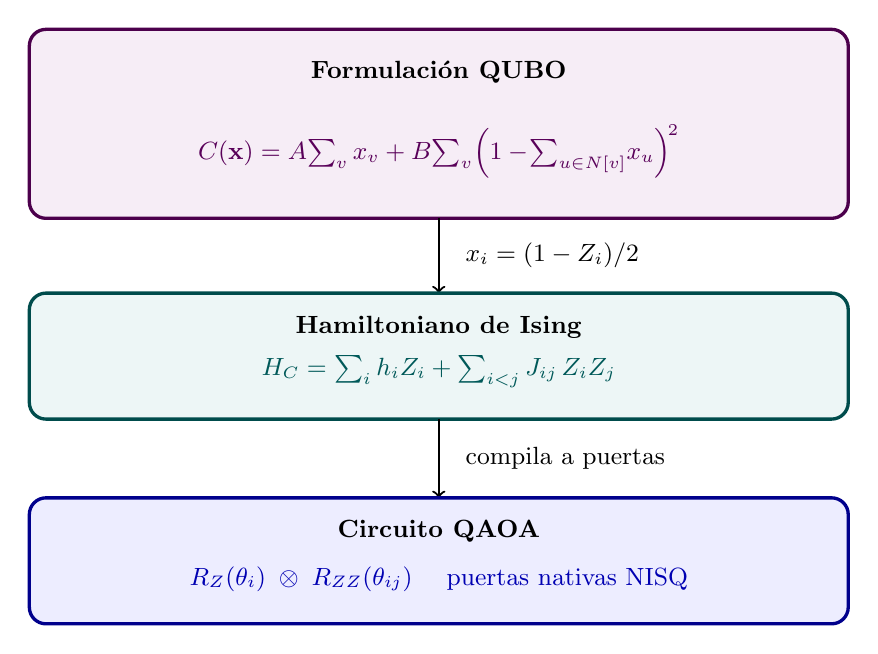
\begin{tikzpicture}[thick, font=\small, node distance=0pt]
  % Bloque 1: QUBO
  \draw[draw=violet!60!black, fill=violet!7, rounded corners=6pt, very thick]
    (-5.2, 1.2) rectangle (5.2, -1.2);
  \node[align=center] at (0, 0.65) {\textbf{Formulación QUBO}};
  \node[align=center, text=violet!70!black] at (0, -0.35)
    {$C(\mathbf{x}) = A\!\sum_{v} x_v + B\!\sum_{v}\!\left(1-\!\sum_{u\in N[v]}\!x_u\right)^{\!2}$};
  % Flecha 1→2
  \draw[->, thick] (0, -1.2) -- (0, -2.15)
    node[midway, right=6pt]{$x_i = (1-Z_i)/2$};
  % Bloque 2: Hamiltoniano de Ising
  \draw[draw=teal!60!black, fill=teal!7, rounded corners=6pt, very thick]
    (-5.2, -2.15) rectangle (5.2, -3.75);
  \node[align=center] at (0, -2.58) {\textbf{Hamiltoniano de Ising}};
  \node[align=center, text=teal!70!black] at (0, -3.15)
    {$H_C = \sum_i h_i Z_i + \sum_{i<j} J_{ij}\, Z_i Z_j$};
  % Flecha 2→3
  \draw[->, thick] (0, -3.75) -- (0, -4.75)
    node[midway, right=6pt]{compila a puertas};
  % Bloque 3: Circuito QAOA
  \draw[draw=blue!55!black, fill=blue!7, rounded corners=6pt, very thick]
    (-5.2, -4.75) rectangle (5.2, -6.35);
  \node[align=center] at (0, -5.18) {\textbf{Circuito QAOA}};
  \node[align=center, text=blue!70!black] at (0, -5.78)
    {$R_Z(\theta_i)\;\otimes\;R_{ZZ}(\theta_{ij})$ \quad puertas nativas NISQ};
\end{tikzpicture}
\caption{Pipeline de compilación del MDS al circuito cuántico. La sustitución $x_i=(1-Z_i)/2$ transforma la función objetivo QUBO en un Hamiltoniano de Ising con términos $Z_i$ (puertas $R_Z$) y $Z_iZ_j$ (puertas $R_{ZZ}$), directamente implementables en hardware NISQ.}
\label{fig:pipeline_qubo_ising}
\end{figure}

\subsection{El loop híbrido cuántico-clásico: arquitectura de referencia NISQ}

El QAOA \citep{farhi2014} implementa el paradigma de optimización variacional mediante la alternancia de dos módulos con responsabilidades estrictamente separadas:

\begin{figure}[ht]
\centering
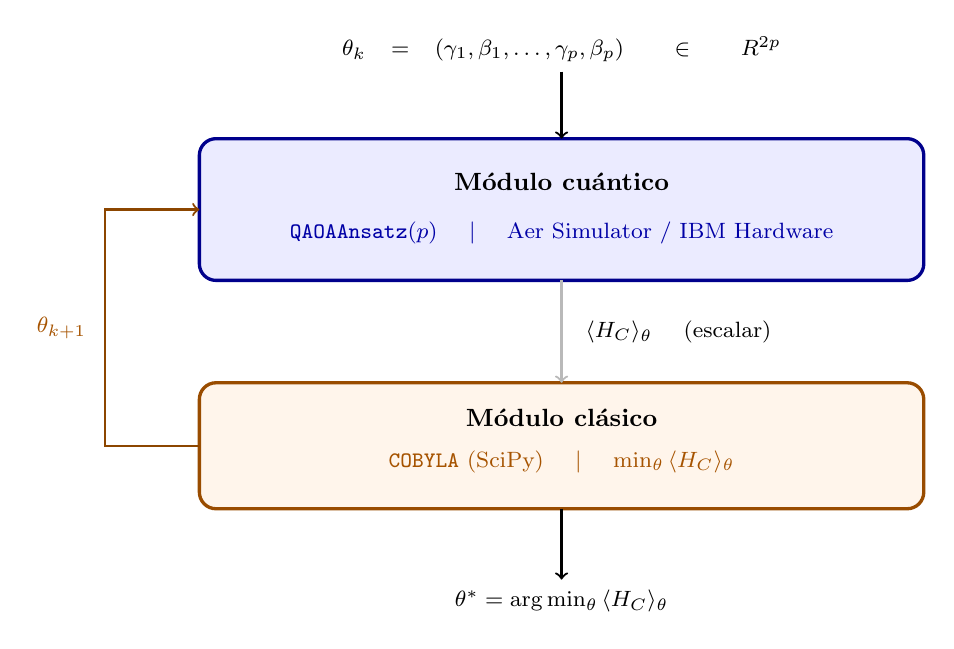
\begin{tikzpicture}[thick, font=\small]
  %--- Módulo cuántico ---
  \draw[draw=blue!55!black, fill=blue!8, rounded corners=6pt, very thick]
    (-4.6, 0.9) rectangle (4.6, -0.9);
  \node[align=center] at (0, 0.35) {\textbf{Módulo cuántico}};
  \node[align=center, font=\footnotesize, text=blue!65!black, text width=8.8cm] at (0, -0.30)
    {\texttt{QAOAAnsatz}$(p)$ \quad $|$ \quad Aer Simulator / IBM Hardware};
  %--- Módulo clásico ---
  \draw[draw=orange!60!black, fill=orange!8, rounded corners=6pt, very thick]
    (-4.6, -2.2) rectangle (4.6, -3.8);
  \node[align=center] at (0, -2.65) {\textbf{Módulo clásico}};
  \node[align=center, font=\footnotesize, text=orange!65!black, text width=8.8cm] at (0, -3.20)
    {\texttt{COBYLA} (SciPy) \quad $|$ \quad $\min_{\boldsymbol{\theta}}\,\langle H_C\rangle_{\boldsymbol{\theta}}$};
  %--- Entrada superior ---
  \draw[->] (0, 1.75) -- (0, 0.90);
  \node[above, font=\footnotesize, align=center, text width=9cm] at (0, 1.75)
    {$\boldsymbol{\theta}_k = (\gamma_1,\beta_1,\ldots,\gamma_p,\beta_p)\;\in\;\mathbb{R}^{2p}$};
  %--- Flecha vertical: energía de Q a C ---
  \draw[->, draw=gray!55] (0, -0.90) -- (0, -2.20)
    node[midway, right=5pt, font=\footnotesize]
    {$\langle H_C \rangle_{\boldsymbol{\theta}}$ \quad (escalar)};
  %--- Flecha de retroalimentación: C devuelve theta a Q ---
  \draw[->, draw=orange!55!black]
    (-4.6, -3.00) -- (-5.8, -3.00) -- (-5.8, 0) -- (-4.6, 0);
  \node[left=3pt, font=\footnotesize, text=orange!65!black] at (-5.8, -1.50)
    {$\boldsymbol{\theta}_{k+1}$};
  %--- Salida inferior ---
  \draw[->] (0, -3.80) -- (0, -4.70);
  \node[below, font=\footnotesize, align=center] at (0, -4.70)
    {$\boldsymbol{\theta}^{*} = \arg\min_{\boldsymbol{\theta}}\,\langle H_C\rangle_{\boldsymbol{\theta}}$};
\end{tikzpicture}
\caption{Arquitectura del loop híbrido cuántico-clásico en QAOA. El módulo cuántico (azul) evalúa la energía esperada $\langle H_C\rangle_{\boldsymbol{\theta}}$ para los parámetros actuales $\boldsymbol{\theta}_k$; el módulo clásico (azul oscuro) los actualiza mediante \texttt{COBYLA} para minimizar esa energía. La interfaz entre módulos se reduce a $2p$ reales de entrada y un único escalar de salida, lo que facilita la integración en cualquier pipeline de optimización existente.}
\label{fig:loop_hibrido}
\end{figure}

\begin{itemize}
  \item \textbf{Módulo cuántico} (Qiskit Aer / hardware IBM): Prepara el estado parametrizado $|\psi(\boldsymbol{\theta})\rangle = U_B(\beta_p)U_C(\gamma_p)\cdots U_B(\beta_1)U_C(\gamma_1)|+\rangle^{\otimes n}$ y evalúa la energía esperada $\langle H_C \rangle_{\boldsymbol{\theta}}$. Los operadores de coste $U_C(\gamma) = e^{-i\gamma H_C}$ se implementan con puertas $R_Z$ y $R_{ZZ}$; los de mezcla $U_B(\beta) = e^{-i\beta \sum_i X_i}$ con rotaciones $R_X$.
  \item \textbf{Módulo clásico} (SciPy COBYLA): Actualiza el vector de ángulos $\boldsymbol{\theta} = (\gamma_1, \ldots, \gamma_p, \beta_1, \ldots, \beta_p) \in \mathbb{R}^{2p}$ para minimizar $\langle H_C \rangle_{\boldsymbol{\theta}}$.
\end{itemize}

\paragraph{Interfaz cuántico-clásica.}
La interfaz entre módulos es \textit{deliberadamente mínima}: el módulo clásico transfiere $2p$ reales al cuántico y recibe un único escalar de retorno:

\begin{table}[ht]
\centering
\caption{Interfaz del loop híbrido QAOA-COBYLA.}
\label{tab:interfaz_hibrida}
\begin{tabular}{lll}
\hline
\textbf{Dirección} & \textbf{Dato} & \textbf{Cardinalidad} \\
\hline
Clásico $\rightarrow$ Cuántico & Ángulos $\boldsymbol{\theta}$ & $2p$ reales \\
Cuántico $\rightarrow$ Clásico & Energía $\langle H_C \rangle_{\boldsymbol{\theta}}$ & 1 escalar \\
Cuántico $\rightarrow$ Clásico & Conteos de medición $\{s: c_s\}$ & $O(\text{shots})$ enteros \\
\hline
\end{tabular}
\end{table}

Esta pequeñísima interfaz implica que QAOA es \textit{directamente integrable} en cualquier pipeline de optimización clásico existente, reemplazando únicamente la función que evalúa el objetivo: el orquestador clásico no necesita conocer los detalles del circuito cuántico.

\subsection{Procedimiento experimental y comparativa clásica}

\begin{enumerate}
  \item \textbf{Referencia exacta}: Fuerza bruta exhaustiva ($2^n = 64$ evaluaciones) y programación lineal entera (ILP con PuLP/CBC), que verifican $D^* = \{\text{Ana, Enrique}\}$.
  \item \textbf{Heurística clásica}: Algoritmo greedy por cobertura incremental —en cada paso se añade el nodo cuyo vecindario cerrado cubre el mayor número de vértices aún no cubiertos— como línea base de tiempo de ejecución.
  \item \textbf{QAOA}: \texttt{QAOAAnsatz} de Qiskit con profundidad $p \in \{1, 2, 3\}$, simulado con el vector de estados exacto (implementación propia en NumPy, verificada contra \texttt{QAOAAnsatz} + \texttt{Statevector} de Qiskit con diferencia máxima de probabilidades de $8\times10^{-16}$). Optimización: 20 reinicios aleatorios de COBYLA con \texttt{maxiter}$=300$ y 6\,000 shots simulados a partir del estado final. Todo el experimento es reproducible con \texttt{python -m qml\_v2.mds\_qaoa} (semilla 42) y escribe sus resultados en \texttt{POCs/data/output/metrics/10\_mds\_qaoa\_*}.
  \item \textbf{Escalabilidad}: Grafos de Erdős-Rényi con $n \in \{6, 8, 10, 12, 15\}$ nodos y densidad 0.45. QAOA, Greedy e ILP se ejecutan en los cinco tamaños; el simulador exacto de QAOA maneja hasta $2^{15}$ amplitudes.
\end{enumerate}

\paragraph{Resultados preliminares.}
Resultados medidos (20 reinicios por profundidad). La probabilidad exacta de medir el óptimo $\{$Ana, Enrique$\}$ es, en media sobre los reinicios, del $2.6\%$ para $p=1$ (máximo $6.1\%$), $3.6\%$ para $p=2$ (máximo $13.0\%$) y $5.7\%$ para $p=3$; solo un reinicio de $p=3$ converge a un buen mínimo local, con $\langle C\rangle=3.78$ y probabilidad $68.8\%$ de medir el óptimo ($68.3\%$ de los 6\,000 shots). La mayoría de reinicios se estanca en $\langle C\rangle\approx 6$ (el coste esperado óptimo es $2$), de modo que, con COBYLA y 300 evaluaciones, QAOA es muy sensible a la inicialización. Aun así, con 6\,000 shots el óptimo se observa con probabilidad $>99\%$ en 12 de 20 reinicios ($p=3$) y, combinando reinicios, el mejor estado muestreado es el óptimo, por lo que se recupera la solución exacta por \emph{selección del estado de menor coste} (no porque el circuito concentre la probabilidad en él). En grafos de Erdős--Rényi con densidad 0.45 ($n\in\{6,8,10,12,15\}$), Greedy e ILP (HiGHS) encuentran el óptimo del MDS en menos de 25 ms en todos los tamaños, mientras que la simulación exacta de QAOA ($p=3$, 20 reinicios) tarda entre 4.8 s ($n=6$) y 31.0 s ($n=15$) con nuestro simulador; QAOA alcanza el óptimo del \emph{QUBO}, que para $n\ge 10$ no es un conjunto dominante del tamaño del MDS (por la penalización cuadrática), y su probabilidad de medir el óptimo cae a $\sim 0.1\%$ para $n=15$. No existe ventaja cuántica en simulación clásica en este rango.

\begin{figure}[!htbp]
\centering
\includegraphics[width=0.97\textwidth]{../POCs/data/output/figures/10_qaoa_histograma_medicion.png}
\caption{Histograma de medición (6\,000 shots) del mejor de 20 reinicios de QAOA con $p=3$ sobre el MDS de 6 nodos; se muestran los 8 estados más frecuentes. El estado azul oscuro \texttt{011000} corresponde al conjunto dominante mínimo óptimo $D^*=\{\text{Ana, Enrique}\}$ (coste QUBO $=2$, verificado por fuerza bruta) y aparece en el 68.3\% de los shots (probabilidad exacta $68.8\%$). El resto son estados sub-óptimos, factibles o no. Las celdas de coste se refieren al valor de la función objetivo QUBO con $A=1$, $B=2$.}
\label{fig:qaoa_histograma}
\end{figure}

\paragraph{Ventajas identificadas.}
\begin{itemize}
  \item El caso ilustra el patrón QAOA-COBYLA en su forma más pura y pedagógicamente transparente, con una cadena completa y verificable: problema de negocio $\rightarrow$ QUBO $\rightarrow$ Hamiltoniano de Ising $\rightarrow$ circuito cuántico $\rightarrow$ loop híbrido $\rightarrow$ medición.
  \item El módulo \texttt{qml\_v2.mds\_qaoa} recibe cualquier lista de nodos y aristas, sin adaptaciones de arquitectura.
  \item La interfaz mínima del loop híbrido ($2p$ parámetros de entrada, 1 escalar de salida) establece el patrón de integración aplicable a los problemas de asignación de SKG Tecnología.
  \item El paso a hardware real de IBM requeriría cambiar el backend de simulación por \texttt{QiskitRuntimeService} + \texttt{EstimatorV2}; no se ha ejecutado en hardware real en este TFM.
\end{itemize}

\paragraph{Limitaciones identificadas.}
\begin{itemize}
  \item En simulación clásica exacta, QAOA no ofrece ventaja en tiempo frente a ILP ni frente a Greedy para $n \leq 15$. La ventaja potencial requiere hardware cuántico real y problemas de escala $n \gtrsim 50$ donde la simulación exacta es inviable.
  \item Con profundidad $p = 1$, la probabilidad media de medir el óptimo es del $2.6\%$ (máximo $6.1\%$ sobre 20 reinicios), insuficiente para uso operativo sin post-procesamiento (selección del menor coste entre las muestras). Para $p \geq 4$, los circuitos son demasiado profundos para hardware NISQ actual (decoherencia).
  \item El parámetro $B$ de la penalización QUBO debe calibrarse para cada familia de instancias: si $B$ es demasiado pequeño, las soluciones infactibles (que no cubren todos los vértices) pueden tener coste QUBO menor que la solución óptima factible.
  \item El número de parámetros a optimizar crece linealmente con $p$ ($2p$ ángulos), lo que aumenta la probabilidad de quedar atrapado en óptimos locales del paisaje de energía; esto motiva el uso de múltiples reinicios aleatorios.
\end{itemize}

\begin{figure}[!htbp]
\centering
\includegraphics[width=0.72\textwidth]{../POCs/data/output/figures/10_mds_grafo_solucion.png}
\caption{Red social de 6 nodos del Caso de uso~7. Los nodos azul oscuro ($D^* = \{\text{Ana, Enrique}\}$) forman el conjunto dominante mínimo de coste 2: contratar a estos dos influencers garantiza que el producto llega a todos los miembros de la red. Las flechas grises indican la relación de cobertura (cada nodo azul tiene al menos un vecino en $D^*$). En QAOA con $p=3$, el mejor reinicio mide este conjunto con probabilidad $68.8\%$ (media sobre 20 reinicios: $5.7\%$).}
\label{fig:mds_grafo_solucion}
\end{figure}

% =====================================================================
\section{Caso de uso 8: Detección de anomalías one-class (OCSVM-ZZ)}
\label{sec:caso8_anomaly}
% =====================================================================

Este caso amplía el marco comparativo a un paradigma \textbf{no supervisado / one-class}, distinto de la detección de fraude. El fraude es, en la práctica, un problema de \emph{clasificación supervisada de clase rara} (etiquetas de fraude en entrenamiento): ese escenario ya queda cubierto por el Caso~1. La detección de anomalías aquí se define como \textbf{novelty detection}: el detector se entrena \emph{solo con inliers} y las etiquetas de outlier se usan exclusivamente en evaluación.

La implementación de referencia vive en el módulo reproducible \texttt{POCs/qml\_v2/anomaly.py} (protocolo QML~v2), alineado con las Tablas~A/B del resto de familias endurecidas.

\subsection{Hipótesis y delimitación}

\begin{itemize}
  \item \textbf{H8a:} cuando la anomalía es densidad o distancia (puntos lejos del soporte de los inliers), IsolationForest / LOF / OCSVM-RBF dominan.
  \item \textbf{H8b:} cuando la anomalía es una \emph{estructura de fase distinta} ocupando el \emph{mismo soporte espacial} que los inliers (\texttt{zz\_phase} ---generador alineado con el mapa ZZ validado en este TFM), el One-Class SVM con kernel de fidelidad ZZ (OCSVM-ZZ) supera a IsolationForest.
  \item \textbf{No-hipótesis:} no se afirma ventaja cuántica genérica sobre anomalías de negocio ni monopolio de ZZ frente a otros feature maps.
\end{itemize}

\subsection{Protocolo experimental justo}

\paragraph{Entrenamiento.} Solo filas con $y=0$ (inliers). El escalado y la PCA (si aplica) se ajustan \textbf{únicamente} sobre esos inliers, evitando fuga de información desde el test o desde outliers conocidos.

\paragraph{Tabla~A (features emparejadas).} Misma matriz ZZ-ready ($n_q=2$ ángulos en $[-\pi,\pi]$) para todos los detectores:
IsolationForest, OCSVM-RBF, LOF y \textbf{OCSVM-ZZ} (kernel de fidelidad sobre \texttt{ZZFeatureMap}).

\paragraph{Tabla~B (negocio).} Mismo split estratificado; los detectores clásicos ven todas las columnas originales. Responde: \textquestiondown{}debe OCSVM-ZZ sustituir IsolationForest en la tabla operativa?

\paragraph{Métricas.} ROC-AUC y average precision sobre el split de test (inliers + outliers). Configuración reportada: $n=160$, 5 repeticiones, contaminación $10\%$, $\nu=0.05$.

\subsection{Datasets}

\begin{itemize}
  \item \texttt{zz\_phase}: datos nativos alineados al mapa ZZ; la clase mayoritaria del generador es inlier y la minoritaria es outlier (mismo soporte en el plano de ángulos).
  \item \texttt{moons} / \texttt{blobs}: manifolds o gaussianas clásicas + outliers sintéticos lejanos.
  \item \texttt{telco\_injected} / \texttt{skg\_injected}: tablas de práctica; se \textbf{descartan} las etiquetas de churn/gravedad y se inyectan spikes lejanos en el espacio de features. SKG sigue siendo dato de práctica, no cliente.
\end{itemize}

\begin{figure}[!htbp]
\centering
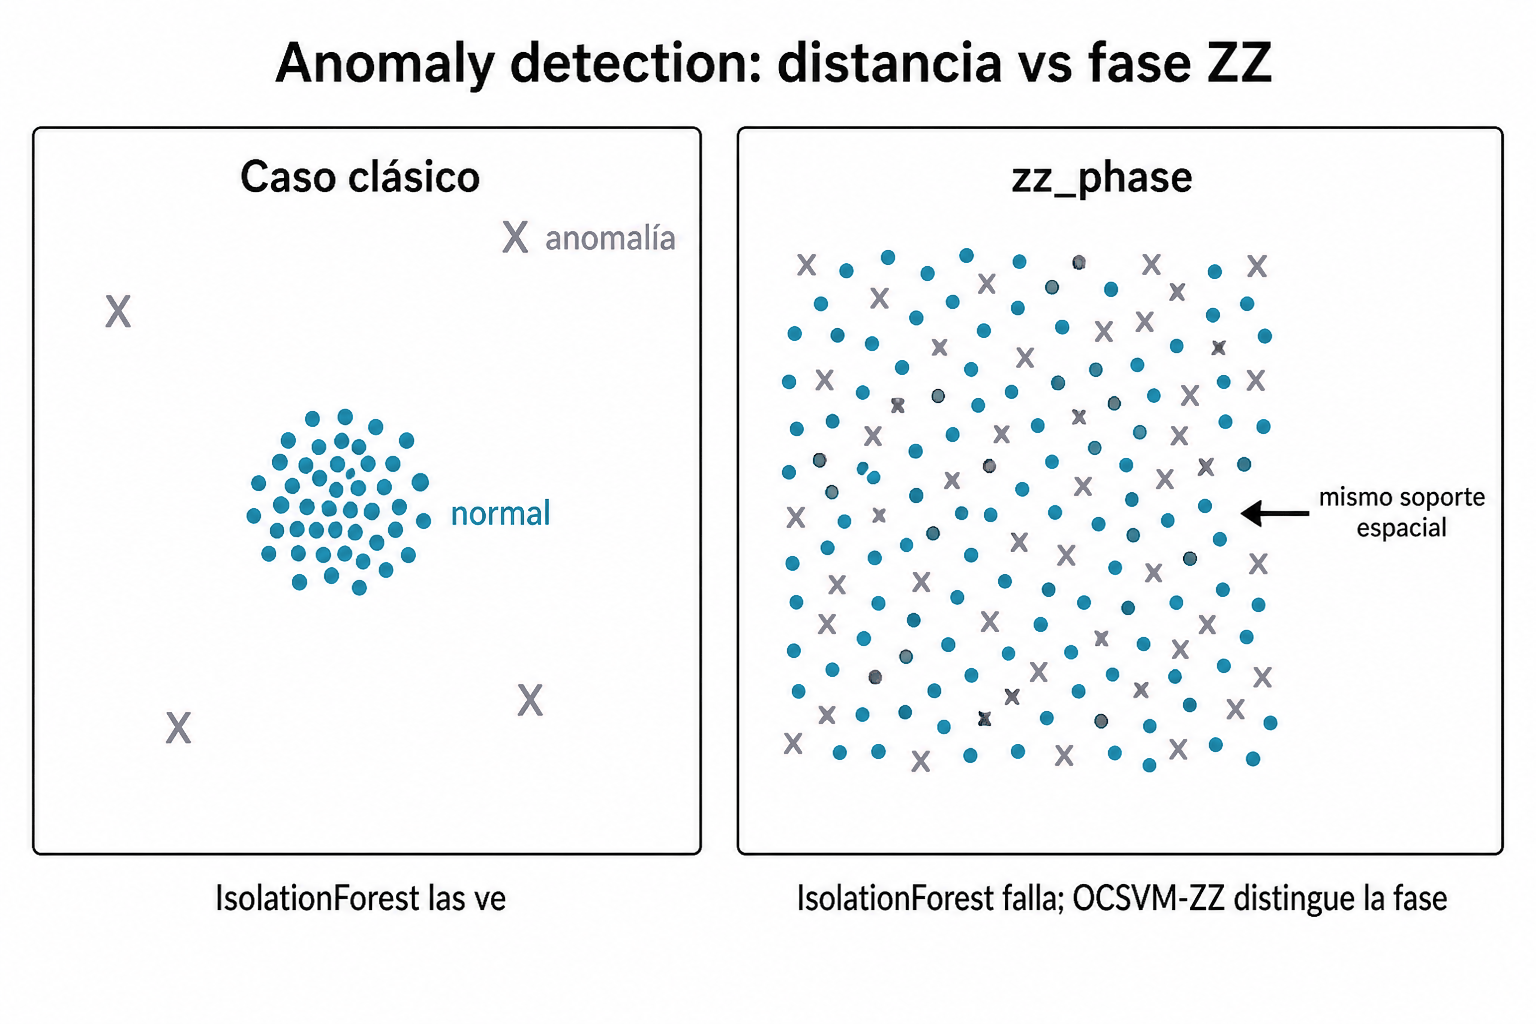
\includegraphics[width=0.98\textwidth]{Imagenes/zz_phase_concept_diagram.png}
\caption{Idea geométrica del Caso~8. Izquierda: anomalía por distancia (IsolationForest la detecta). Derecha: anomalía por estructura de fase alineada al feature map, mismo soporte espacial (IsolationForest falla; OCSVM-ZZ puede separar ---mapa validado: ZZ).}
\label{fig:anomaly_concept}
\end{figure}

\begin{figure}[!htbp]
\centering
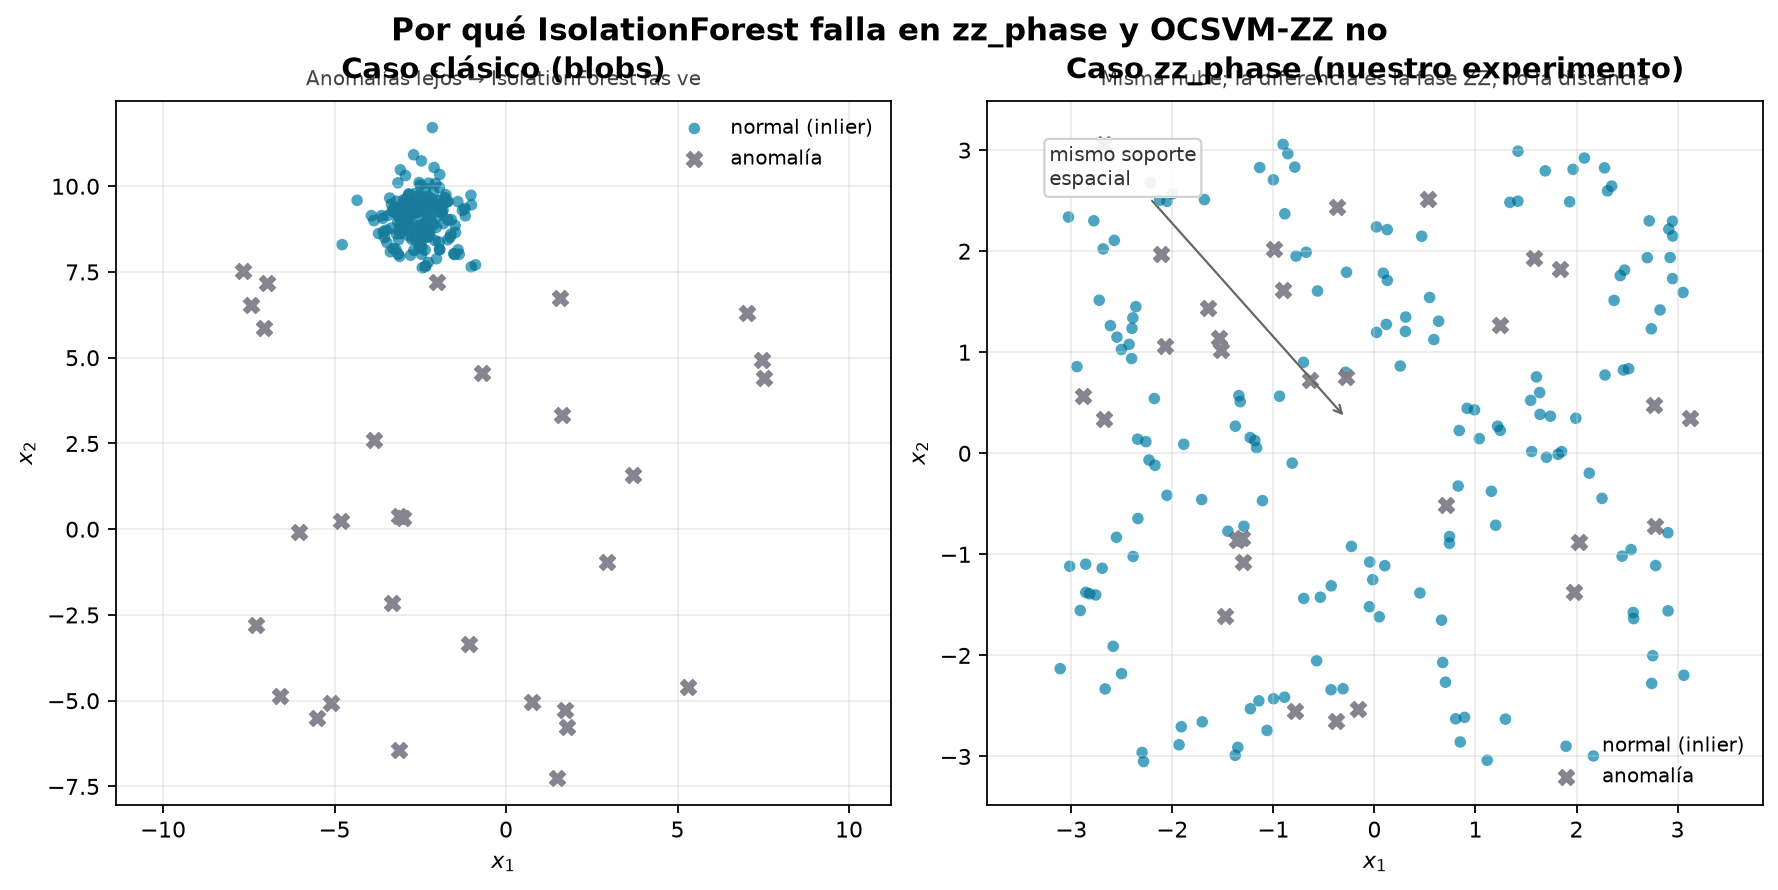
\includegraphics[width=0.98\textwidth]{Imagenes/zz_phase_vs_blobs_anomaly.png}
\caption{Datos reales del generador QML~v2. En \texttt{blobs} las anomalías están lejos del blob de inliers; en \texttt{zz\_phase} normales y anomalías comparten la misma nube en el plano de ángulos.}
\label{fig:anomaly_support}
\end{figure}

% =====================================================================
\section{Caso de uso 9: Forecasting one-step por lags (QK-SVR)}
\label{sec:caso9_timeseries}
% =====================================================================

Este caso extiende la familia de kernels a \textbf{series temporales} con un protocolo justo de predicción un paso adelante: $y_t$ se estima únicamente a partir de una ventana de los valores anteriores (\textit{lags}). No es una comparación frente a ARIMA o Prophet: la pregunta es si un kernel ZZ sobre el vector de lags supera a regresores clásicos que ven \emph{los mismos lags}. Implementación: \texttt{POCs/qml\_v2/timeseries.py}; cuaderno: Notebook~12.

\subsection{Protocolo}

\begin{itemize}
  \item \textbf{Tabla~A:} QK-SVR (kernel de fidelidad ZZ, $n_q=2$ qubits), Ridge, SVR-RBF y Gradient Boosting reciben las mismas $n_{\mathrm{lags}}=n_q=2$ variables.
  \item \textbf{Tabla~B:} los clásicos reciben además 4 lags adicionales, media y desviación de la ventana y, en la serie SKG, la hora del día en codificación cíclica (mismas muestras de entrenamiento).
  \item \textbf{División temporal:} el 70\,\% inicial de la serie es entrenamiento y el 30\,\% final es prueba, sin barajar, de modo que no hay fuga de información del futuro. 5 repeticiones.
  \item \textbf{Referencias ingenuas:} el MAE de la \emph{persistencia} ($\hat y_t=y_{t-1}$) y el de predecir la media del entrenamiento sobre las mismas ventanas de prueba, para interpretar el error absoluto de cada modelo.
\end{itemize}

\subsection{Datasets e hipótesis}

La Figura~\ref{fig:ts_datasets} muestra los tres conjuntos.

\begin{itemize}
  \item \texttt{zz\_lag} (cuántico-nativo): pares de lags $(y_{t-2},y_{t-1})$ en $[-\pi,\pi]^2$ y objetivo $y_t=\langle ZZ\rangle$ del estado preparado por el mapa ZZ con esos ángulos, de modo que target y feature map están alineados por construcción. Los pares son independientes entre sí: es el control nativo del protocolo, no una serie con dinámica propia. Cada repetición toma 160 ventanas de un conjunto de 320.
  \item \texttt{sine} (referencia sintética): $\sin(2\pi t/24)+0.3\sin(2\pi t/7)$ más ruido gaussiano ($\sigma=0.15$), 480 puntos; cada repetición toma una ventana contigua de 160. Periodicidad clásica.
  \item \texttt{skg\_speed} (SKG, datos de práctica): velocidad de los corredores viales de Bogotá (\texttt{bctraveltimes\_history.csv}; 582 corredores con una lectura cada 5 minutos durante 12~h). Cada repetición usa un corredor distinto (los 5 con más lecturas, 144 cada uno, 138 ventanas), de forma que las repeticiones no reutilizan la misma serie.
\end{itemize}

\begin{figure}[ht]
\centering
\includegraphics[width=\textwidth]{../POCs/data/output/figures/12_series_datasets.png}
\caption{Datasets del Caso~9. Izquierda: \texttt{zz\_lag}, con los dos lags como ejes y el objetivo $\langle ZZ\rangle$ como color. Centro y derecha: \texttt{sine} y un corredor de \texttt{skg\_speed}, con la zona de prueba (futuro) sombreada. Fuente: Notebook~12.}
\label{fig:ts_datasets}
\end{figure}

\subsection{Resultados (Tabla~A)}

\begin{table}[ht]
\centering
\small
\begin{tabular}{llcc}
\hline
\textbf{Dataset} & \textbf{Mejor Tabla~A} & \textbf{MAE} & \textbf{Lectura} \\
\hline
\texttt{zz\_lag} & \textbf{QK-SVR-ZZ} & \textbf{0.056} frente a Ridge 0.414 & Target $=\langle ZZ\rangle$ \\
\texttt{sine} & SVR-RBF & 0.260 frente a QK-SVR 0.662 & Periodicidad clásica \\
\texttt{skg\_speed} & Ridge & 2.80 frente a QK-SVR 13.59 & Práctica; clásico \\
\hline
\end{tabular}
\caption{Caso~9. MAE en test (media de 5 repeticiones). Ventaja solo cuando el generador del target está alineado con el feature map (aquí ZZ en \texttt{zz\_lag}). Fuente: \texttt{fair\_timeseries\_*.csv}.}
\label{tab:timeseries_dev}
\end{table}

\paragraph{Lectura.}
Mismo principio transversal que en clasificación y anomalías: no ``ZZ gana en series'', sino ``el mapa alineado gana; ZZ es el que medimos''. Fuera del régimen nativo el kernel ZZ de 2 qubits no extrae señal: su MAE coincide con el de predecir la media del entrenamiento ($0.662$ frente a $0.658$ en \texttt{sine}; $13.59$ frente a $13.61$ en \texttt{skg\_speed}), mientras que Ridge se sitúa en el nivel de la persistencia ($2.80$ frente a $2.75$ en SKG). En el corredor SKG la opción operativa es, por tanto, un modelo lineal sobre lags (o la propia persistencia); añadir variables clásicas (Tabla~B) no mejora el resultado con series de solo 138 ventanas.

% =====================================================================
\section{Prototipo de arquitectura híbrida cuántico-clásica}
\label{sec:prototipo_hibrido}
% =====================================================================

Los nueve casos de uso desarrollados en este capítulo ilustran, cada uno desde un ángulo diferente, la misma idea estructural: los algoritmos cuánticos variacionales de la era NISQ no reemplazan a los clásicos sino que se integran con ellos en un \textbf{pipeline híbrido} donde cada parte hace lo que mejor sabe hacer. Esta sección sintetiza ese patrón de diseño en forma de prototipo arquitectónico aplicable a un entorno empresarial como SKG Tecnología.

\subsection{Principio de diseño: separación de responsabilidades}

La arquitectura híbrida cuántico-clásica se sustenta en una premisa simple: el módulo cuántico resuelve la parte del problema que es difícil para los computadores clásicos —la exploración de espacios de búsqueda exponencialmente grandes o la evaluación de kernels en espacios de Hilbert de alta dimensión—, mientras que el módulo clásico orquesta el flujo, pre-procesa los datos, ejecuta la optimización de parámetros y toma la decisión final a partir de los resultados cuánticos.

\subsection{Flujo de decisión: cuándo activar el módulo cuántico}

No todos los problemas se benefician del módulo cuántico. La Tabla~\ref{tab:flujo_hibrido} resume el criterio de activación según el tipo de problema.

\begin{table}[ht]
\centering
\small
\begin{tabular}{>{\raggedright\arraybackslash}p{3.2cm}>{\raggedright\arraybackslash}p{3.2cm}>{\raggedright\arraybackslash}p{3.5cm}>{\raggedright\arraybackslash}p{3.0cm}}
\hline
\textbf{Tipo de problema} & \textbf{Criterio de activación} & \textbf{Módulo cuántico} & \textbf{Módulo clásico} \\
\hline
Clasificación / Regresión &
$\mathcal{Q}(\mathcal{D}) > 0$ (score de cuanticidad positivo) &
QSVM / QK-SVR (kernel cuántico) &
Gradient Boosting como fallback \\
\hline
Detección de anomalías (one-class) &
Anomalía alineada al feature map (p.\,ej.\ \texttt{zz\_phase}, $\mathcal{Q}>0$) &
OCSVM-ZZ (u otro kernel si el mapa cambia) &
IsolationForest / LOF como default \\
\hline
Forecasting (lags) &
Target alineado al mapa (p.\,ej.\ \texttt{zz\_lag}) &
QK-SVR (ZZ u otro) &
Ridge / SVR-RBF / GB \\
\hline
Optimización combinatoria / TSP &
QUBO factible; $n_{\text{vars}}$ compatible con hardware &
QAOA ($p \geq 1$) &
NN+2-opt / ILP / verificación \\
\hline
Caso general &
$\mathcal{Q}(\mathcal{D}) \leq 0$ o $n_{\text{vars}} > 50$ &
No se activa &
Pipeline clásico estándar \\
\hline
\end{tabular}
\caption{Criterio de activación del módulo cuántico en la arquitectura híbrida propuesta.}
\label{tab:flujo_hibrido}
\end{table}

\subsection{Arquitectura de referencia}

El prototipo conceptual se articula en cuatro capas:

\begin{enumerate}
  \item \textbf{Capa de diagnóstico} (\textit{clásica}): Calcula el score $\mathcal{Q}(\mathcal{D})$ o verifica si el problema es formulable como QUBO. Decide si el módulo cuántico es pertinente. Esta capa emplea exclusivamente computación clásica y tiene coste lineal en el tamaño del dataset.

  \item \textbf{Capa de preprocesamiento} (\textit{clásica}): Aplica, si es necesario, el Framework QCR (re-uploading, rotación, reducción dimensional) para maximizar la compatibilidad cuántica de los datos. Para problemas de optimización, construye la matriz QUBO y la traduce a \texttt{SparsePauliOp}.

  \item \textbf{Capa de cómputo cuántico} (\textit{cuántica}): Ejecuta el circuito cuántico — kernel cuántico (para clasificación/regresión) o QAOA/VQE (para optimización) — sobre el simulador Aer o sobre hardware IBM Quantum. Devuelve la energía esperada (optimización) o los valores del kernel (clasificación).

  \item \textbf{Capa de decisión} (\textit{clásica}): Integra el resultado cuántico en el pipeline existente: el optimizador COBYLA actualiza los parámetros del circuito (loop híbrido), o el clasificador SVM toma la predicción final a partir de la matriz de kernel cuántico. El resultado final es siempre una salida clásica (asignación, etiqueta, regresión).
\end{enumerate}

\begin{figure}[!htbp]
\centering
\begin{tikzpicture}[thick, font=\small,
    capa/.style={rectangle, rounded corners=5pt, very thick,
                 minimum width=0.92\textwidth, text width=0.88\textwidth,
                 align=center, inner sep=7pt},
    arr/.style={->, very thick}]

  % --- Capa 1: Diagnóstico ---
  \node[capa, draw=gray!60!black, fill=gray!10] (c1) {
    \textbf{Capa 1 — Diagnóstico} \normalfont\footnotesize(clásica)\\[3pt]
    {\scriptsize\color{gray!55!black}%
     Calcula $\mathcal{Q}(\mathcal{D})$ / verifica formulación QUBO
     \;$\rightarrow$\; \textquestiondown{}activar módulo cuántico?}
  };

  % --- Capa 2: Preprocesamiento ---
  \node[capa, draw=orange!55!black, fill=orange!7, below=0.5cm of c1] (c2) {
    \textbf{Capa 2 — Preprocesamiento} \normalfont\footnotesize(clásica)\\[3pt]
    {\scriptsize\color{orange!65!black}%
     Framework QCR: re-uploading / rotación / QUBO $\rightarrow$ \texttt{SparsePauliOp}}
  };

  % --- Capa 3: Cómputo cuántico ---
  \node[capa, draw=blue!55!black, fill=blue!7, below=0.5cm of c2] (c3) {
    \textbf{Capa 3 — Cómputo cuántico} \normalfont\footnotesize(cuántica)\\[3pt]
    {\scriptsize\color{blue!65!black}%
     Kernel cuántico (QSVM) \;$|$\; QAOA/VQE \quad Aer / IBM Quantum Hardware}
  };

  % --- Capa 4: Decisión ---
  \node[capa, draw=teal!55!black, fill=teal!7, below=0.5cm of c3] (c4) {
    \textbf{Capa 4 — Decisión} \normalfont\footnotesize(clásica)\\[3pt]
    {\scriptsize\color{teal!65!black}%
     SVM / COBYLA actualiza $\boldsymbol{\theta}$
     \;$\rightarrow$\; salida: etiqueta / asignación / regresión}
  };

  % --- Flechas ---
  \draw[arr] (c1.south) -- node[right=5pt, font=\scriptsize]{Sí: continuar} (c2.north);
  \draw[arr] (c2.south) -- (c3.north);
  \draw[arr] (c3.south) -- (c4.north);
  \draw[arr] (c4.south) -- ++(0,-0.55)
    node[below, font=\scriptsize]{Resultado clásico final};

\end{tikzpicture}
\caption{Arquitectura de referencia del prototipo híbrido en cuatro capas. Las capas 1, 2 y 4 son puramente clásicas; la capa 3 es el único punto de ejecución cuántica. Esta separación permite desactivar el módulo cuántico sin modificar el resto del pipeline.}
\label{fig:arquitectura_cuatro_capas}
\end{figure}

\subsection{Posicionamiento como herramienta complementaria}

Una reflexión importante que emerge del análisis experimental es que la arquitectura híbrida no tiene sentido como sistema aislado, sino como \textbf{herramienta adicional dentro del stack tecnológico existente}. En el caso de SKG Tecnología, el sistema actual de gestión de incidentes y asignación de recursos seguiría operando con sus algoritmos clásicos consolidados. El módulo cuántico solo se activaría en los subproblemas donde se demuestre una ventaja medible. En los experimentos de este trabajo eso se cumple de forma condicional en clasificación con estructura cuántica (Caso~1) y no se cumple en optimización combinatoria de asignación de recursos, donde la formulación QUBO es natural y el QAOA con $p=1$ recupera el óptimo, pero empata con los métodos exactos (Caso~3).

La adopción de esta arquitectura no requiere reemplazar ningún sistema existente, sino añadir un módulo con interfaz bien definida ---$2p$ parámetros de entrada, 1 escalar de salida--- que puede ser desactivado sin consecuencias si el hardware cuántico no está disponible o si el problema no cumple los criterios de activación de la Tabla~\ref{tab:flujo_hibrido}.
